%%%% using 'arara' 4.0
% arara: pdflatex: {synctex: yes, interaction: nonstopmode}
% arara: bibtex
% arara: latexindent
% arara: pdflatex: {synctex: yes, interaction: nonstopmode}
% arara: pdflatex: {synctex: yes, interaction: nonstopmode}

%% bare_jrnl.tex
%% V1.4b
%% 2015/08/26
%% by Michael Shell
%% see http://www.michaelshell.org/
%% for current contact information.
%%
%% This is a skeleton file demonstrating the use of IEEEtran.cls
%% (requires IEEEtran.cls version 1.8b or later) with an IEEE
%% journal paper.
%%
%% Support sites:
%% http://www.michaelshell.org/tex/ieeetran/
%% http://www.ctan.org/pkg/ieeetran
%% and
%% http://www.ieee.org/

%%*************************************************************************
%% Legal Notice:
%% This code is offered as-is without any warranty either expressed or
%% implied; without even the implied warranty of MERCHANTABILITY or
%% FITNESS FOR A PARTICULAR PURPOSE!
%% User assumes all risk.
%% In no event shall the IEEE or any contributor to this code be liable for
%% any damages or losses, including, but not limited to, incidental,
%% consequential, or any other damages, resulting from the use or misuse
%% of any information contained here.
%%
%% All comments are the opinions of their respective authors and are not
%% necessarily endorsed by the IEEE.
%%
%% This work is distributed under the LaTeX Project Public License (LPPL)
%% ( http://www.latex-project.org/ ) version 1.3, and may be freely used,
%% distributed and modified. A copy of the LPPL, version 1.3, is included
%% in the base LaTeX documentation of all distributions of LaTeX released
%% 2003/12/01 or later.
%% Retain all contribution notices and credits.
%% ** Modified files should be clearly indicated as such, including  **
%% ** renaming them and changing author support contact information. **
%%*************************************************************************

% *** Authors should verify (and, if needed, correct) their LaTeX system  ***
% *** with the testflow diagnostic prior to trusting their LaTeX platform ***
% *** with production work. The IEEE's font choices and paper sizes can   ***
% *** trigger bugs that do not appear when using other class files.       ***                          ***
% The testflow support page is at:
% http://www.michaelshell.org/tex/testflow/

\documentclass[letterpaper, peerreview]{IEEEtran}
%
% If IEEEtran.cls has not been installed into the LaTeX system files,
% manually specify the path to it like:
% \documentclass[journal]{../sty/IEEEtran}

% Some very useful LaTeX packages include:
% (uncomment the ones you want to load)

% *** MISC UTILITY PACKAGES ***
%
%\usepackage{ifpdf}
% Heiko Oberdiek's ifpdf.sty is very useful if you need conditional
% compilation based on whether the output is pdf or dvi.
% usage:
% \ifpdf
%   % pdf code
% \else
%   % dvi code
% \fi
% The latest version of ifpdf.sty can be obtained from:
% http://www.ctan.org/pkg/ifpdf
% Also, note that IEEEtran.cls V1.7 and later provides a builtin
% \ifCLASSINFOpdf conditional that works the same way.
% When switching from latex to pdflatex and vice-versa, the compiler may
% have to be run twice to clear warning/error messages.

% *** CITATION PACKAGES ***
%
\usepackage{cite}
\usepackage[hidelinks]{hyperref}
% cite.sty was written by Donald Arseneau
% V1.6 and later of IEEEtran pre-defines the format of the cite.sty package
%\cite{} output to follow that of the IEEE. Loading the cite package will
% result in citation numbers being automatically sorted and properly
% 'compressed/ranged'. e.g., [1], [9], [2], [7], [5], [6] without using
% cite.sty will become [1], [2], [5]--[7], [9] using cite.sty. cite.sty's
%\cite will automatically add leading space, if needed. Use cite.sty's
% noadjust option (cite.sty V3.8 and later) if you want to turn this off
% such as if a citation ever needs to be enclosed in parenthesis.
% cite.sty is already installed on most LaTeX systems. Be sure and use
% version 5.0 (2009-03-20) and later if using hyperref.sty.
% The latest version can be obtained at:
% http://www.ctan.org/pkg/cite
% The documentation is contained in the cite.sty file itself.

% *** GRAPHICS RELATED PACKAGES ***
%
\ifCLASSINFOpdf{}
  \usepackage[pdftex]{graphicx}
  % declare the path(s) where your graphic files are
  \graphicspath{{./pdf/}{./jpg/}}
  % and their extensions so you won't have to specify these with
  % every instance of \includegraphics
  \DeclareGraphicsExtensions{.pdf,.jpg,.png}
\else
  % or other class option (dvipsone, dvipdf, if not using dvips). graphicx
  % will default to the driver specified in the system graphics.cfg if no
  % driver is specified.
  % \usepackage[dvips]{graphicx}
  % declare the path(s) where your graphic files are
  % \graphicspath{{../eps/}}
  % and their extensions so you won't have to specify these with
  % every instance of \includegraphics
  % \DeclareGraphicsExtensions{.eps}
\fi
% graphicx was written by David Carlisle and Sebastian Rahtz. It is
% required if you want graphics, photos, etc. graphicx.sty is already
% installed on most LaTeX systems. The latest version and documentation
% can be obtained at:
% http://www.ctan.org/pkg/graphicx
% Another good source of documentation is 'Using Imported Graphics in
% LaTeX2e' by Keith Reckdahl which can be found at:
% http://www.ctan.org/pkg/epslatex
%
% latex, and pdflatex in dvi mode, support graphics in encapsulated
% postscript (.eps) format. pdflatex in pdf mode supports graphics
% in .pdf, .jpeg, .png and .mps (metapost) formats. Users should ensure
% that all non-photo figures use a vector format (.eps, .pdf, .mps) and
% not a bitmapped formats (.jpeg, .png). The IEEE frowns on bitmapped formats
% which can result in 'jaggedy'/blurry rendering of lines and letters as
% well as large increases in file sizes.
%
% You can find documentation about the pdfTeX application at:
% http://www.tug.org/applications/pdftex

% *** MATH PACKAGES ***
%
\usepackage{amsmath}
% A popular package from the American Mathematical Society that provides
% many useful and powerful commands for dealing with mathematics.
%
% Note that the amsmath package sets \interdisplaylinepenalty to 10000
% thus preventing page breaks from occurring within multiline equations. Use:
%\interdisplaylinepenalty=2500
% after loading amsmath to restore such page breaks as IEEEtran.cls normally
% does. amsmath.sty is already installed on most LaTeX systems. The latest
% version and documentation can be obtained at:
% http://www.ctan.org/pkg/amsmath

% *** SPECIALIZED LIST PACKAGES ***
%
%\usepackage{algorithmic}
% algorithmic.sty was written by Peter Williams and Rogerio Brito.
% This package provides an algorithmic environment fo describing algorithms.
% You can use the algorithmic environment in-text or within a figure
% environment to provide for a floating algorithm. Do NOT use the algorithm
% floating environment provided by algorithm.sty (by the same authors) or
% algorithm2e.sty (by Christophe Fiorio) as the IEEE does not use dedicated
% algorithm float types and packages that provide these will not provide
% correct IEEE style captions. The latest version and documentation of
% algorithmic.sty can be obtained at:
% http://www.ctan.org/pkg/algorithms
% Also of interest may be the (relatively newer and more customizable)
% algorithmicx.sty package by Szasz Janos:
% http://www.ctan.org/pkg/algorithmicx

% *** ALIGNMENT PACKAGES ***
%
%\usepackage{array}
% Frank Mittelbach's and David Carlisle's array.sty patches and improves
% the standard LaTeX2e array and tabular environments to provide better
% appearance and additional user controls. As the default LaTeX2e table
% generation code is lacking to the point of almost being broken with
% respect to the quality of the end results, all users are strongly
% advised to use an enhanced (at the very least that provided by array.sty)
% set of table tools. array.sty is already installed on most systems. The
% latest version and documentation can be obtained at:
% http://www.ctan.org/pkg/array

% IEEEtran contains the IEEEeqnarray family of commands that can be used to
% generate multiline equations as well as matrices, tables, etc., of high
% quality.

% *** SUBFIGURE PACKAGES ***
%\ifCLASSOPTIONcompsoc
%  \usepackage[caption=false,font=normalsize,labelfont=sf,textfont=sf]{subfig}
%\else
%  \usepackage[caption=false,font=footnotesize]{subfig}
%\fi
% subfig.sty, written by Steven Douglas Cochran, is the modern replacement
% for subfigure.sty, the latter of which is no longer maintained and is
% incompatible with some LaTeX packages including fixltx2e. However,
% subfig.sty requires and automatically loads Axel Sommerfeldt's caption.sty
% which will override IEEEtran.cls' handling of captions and this will result
% in non-IEEE style figure/table captions. To prevent this problem, be sure
% and invoke subfig.sty's 'caption=false' package option (available since
% subfig.sty version 1.3, 2005/06/28) as this is will preserve IEEEtran.cls
% handling of captions.
% Note that the Computer Society format requires a larger sans serif font
% than the serif footnote size font used in traditional IEEE formatting
% and thus the need to invoke different subfig.sty package options depending
% on whether compsoc mode has been enabled.
%
% The latest version and documentation of subfig.sty can be obtained at:
% http://www.ctan.org/pkg/subfig

% *** FLOAT PACKAGES ***
%
%\usepackage{fixltx2e}
% fixltx2e, the successor to the earlier fix2col.sty, was written by
% Frank Mittelbach and David Carlisle. This package corrects a few problems
% in the LaTeX2e kernel, the most notable of which is that in current
% LaTeX2e releases, the ordering of single and double column floats is not
% guaranteed to be preserved. Thus, an unpatched LaTeX2e can allow a
% single column figure to be placed prior to an earlier double column
% figure.
% Be aware that LaTeX2e kernels dated 2015 and later have fixltx2e.sty's
% corrections already built into the system in which case a warning will
% be issued if an attempt is made to load fixltx2e.sty as it is no longer
% needed.
% The latest version and documentation can be found at:
% http://www.ctan.org/pkg/fixltx2e

%\usepackage{stfloats}
% stfloats.sty was written by Sigitas Tolusis. This package gives LaTeX2e
% the ability to do double column floats at the bottom of the page as well
% as the top. (e.g., '\begin{figure*}[!b]' is not normally possible in
% LaTeX2e). It also provides a command:
%\fnbelowfloat
% to enable the placement of footnotes below bottom floats (the standard
% LaTeX2e kernel puts them above bottom floats). This is an invasive package
% which rewrites many portions of the LaTeX2e float routines. It may not work
% with other packages that modify the LaTeX2e float routines. The latest
% version and documentation can be obtained at:
% http://www.ctan.org/pkg/stfloats
% Do not use the stfloats baselinefloat ability as the IEEE does not allow
% \baselineskip to stretch. Authors submitting work to the IEEE should note
% that the IEEE rarely uses double column equations and that authors should try
% to avoid such use. Do not be tempted to use the cuted.sty or midfloat.sty
% packages (also by Sigitas Tolusis) as the IEEE does not format its papers in
% such ways.
% Do not attempt to use stfloats with fixltx2e as they are incompatible.
% Instead, use Morten Hogholm'a dblfloatfix which combines the features
% of both fixltx2e and stfloats:
%
% \usepackage{dblfloatfix}
% The latest version can be found at:
% http://www.ctan.org/pkg/dblfloatfix

%\ifCLASSOPTIONcaptionsoff
%  \usepackage[nomarkers]{endfloat}
% \let\MYoriglatexcaption\caption
% \renewcommand{\caption}[2][\relax]{\MYoriglatexcaption[#2]{#2}}
%\fi
% endfloat.sty was written by James Darrell McCauley, Jeff Goldberg and
% Axel Sommerfeldt. This package may be useful when used in conjunction with
% IEEEtran.cls'  captionsoff option. Some IEEE journals/societies require that
% submissions have lists of figures/tables at the end of the paper and that
% figures/tables without any captions are placed on a page by themselves at
% the end of the document. If needed, the draftcls IEEEtran class option or
% \CLASSINPUTbaselinestretch interface can be used to increase the line
% spacing as well. Be sure and use the nomarkers option of endfloat to
% prevent endfloat from 'marking' where the figures would have been placed
% in the text. The two hack lines of code above are a slight modification of
% that suggested by in the endfloat docs (section 8.4.1) to ensure that
% the full captions always appear in the list of figures/tables - even if
% the user used the short optional argument of \caption[]{}.
% IEEE papers do not typically make use of \caption[]'s optional argument,
% so this should not be an issue. A similar trick can be used to disable
% captions of packages such as subfig.sty that lack options to turn off
% the subcaptions:
% For subfig.sty:
% \let\MYorigsubfloat\subfloat
% \renewcommand{\subfloat}[2][\relax]{\MYorigsubfloat[]{#2}}
% However, the above trick will not work if both optional arguments of
% the \subfloat command are used. Furthermore, there needs to be a
% description of each subfigure *somewhere* and endfloat does not add
% subfigure captions to its list of figures. Thus, the best approach is to
% avoid the use of subfigure captions (many IEEE journals avoid them anyway)
% and instead reference/explain all the subfigures within the main caption.
% The latest version of endfloat.sty and its documentation can obtained at:
% http://www.ctan.org/pkg/endfloat
%
% The IEEEtran \ifCLASSOPTIONcaptionsoff conditional can also be used
% later in the document, say, to conditionally put the References on a
% page by themselves.

% *** PDF, URL AND HYPERLINK PACKAGES ***
%
\usepackage{url}
% url.sty was written by Donald Arseneau. It provides better support for
% handling and breaking URLs. url.sty is already installed on most LaTeX
% systems. The latest version and documentation can be obtained at:
% http://www.ctan.org/pkg/url
% Basically, \url{my_url_here}.

% *** Do not adjust lengths that control margins, column widths, etc. ***
% *** Do not use packages that alter fonts (such as pslatex).         ***
% There should be no need to do such things with IEEEtran.cls V1.6 and later.
% (Unless specifically asked to do so by the journal or conference you plan
% to submit to, of course. )

% correct bad hyphenation here
\hyphenation{op-tical net-works semi-conduc-tor}

\usepackage[nolist]{acronym}

\usepackage{booktabs}
\usepackage{adjustbox}

\begin{document}
%
% paper title
% Titles are generally capitalized except for words such as a, an, and, as,
% at, but, by, for, in, nor, of, on, or, the, to and up, which are usually
% not capitalized unless they are the first or last word of the title.
% Linebreaks \\ can be used within to get better formatting as desired.
% Do not put math or special symbols in the title.
\title{Supporting Ecological Decision Making Using Feature-Selection and Variable Importance}
\IEEEpeerreviewmaketitle{Supporting Ecological Decision Making Using Feature-Selection and Variable Importance}
%
%
% author names and IEEE memberships
% note positions of commas and nonbreaking spaces ( ~ ) LaTeX will not break
% a structure at a ~ so this keeps an author's name from being broken across
% two lines.
% use \thanks{} to gain access to the first footnote area
% a separate \thanks must be used for each paragraph as LaTeX2e's \thanks
% was not built to handle multiple paragraphs
%

% suppress 'underfull hbox' warnings
\hbadness=99999

\author{Patrick~Schratz,~\IEEEmembership{Member,~IEEE,}
	Jannes~Muenchow,~\IEEEmembership{Member,~IEEE,}
	Eugenia Iturritxa,~\IEEEmembership{Member,~IEEE,}
	José Cortés,~\IEEEmembership{Member,~IEEE,}
	Bernd~Bischl,~\IEEEmembership{Member,~IEEE,}
	and Alexander~Brenning,~\IEEEmembership{Member,~IEEE}
	\thanks{P. Schratz, J. Muenchow, J. Cortés and A. Brenning are with the Department
		of Geography, GIScience group, Friedrich-Schiller-University of Jena, Germany.}% <-this % stops a space
	\thanks{B. Bischl is head of the computational statistics group at the Department of Statistics, Ludwig-Maximilian-University Munich.}% <-this % stops a space
	\thanks{E. Iturritxa is with NEIKER Tecnalia, Vitoria-Gasteiz, Arab, Spain.}% <-this % stops a space
	%\thanks{Manuscript received April 19, 2005; revised August 26, 2015.}
}

% note the % following the last \IEEEmembership and also \thanks -
% these prevent an unwanted space from occurring between the last author name
% and the end of the author line. i.e., if you had this:
%
% \author{....lastname \thanks{...} \thanks{...} }
%                     ^------------^------------^----Do not want these spaces!
%
% a space would be appended to the last name and could cause every name on that
% line to be shifted left slightly. This is one of those 'LaTeX things'. For
% instance, '\textbf{A} \textbf{B}' will typeset as 'A B' not 'AB'. To get
% 'AB' then you have to do: '\textbf{A}\textbf{B}'
% \thanks is no different in this regard, so shield the last } of each \thanks
% that ends a line with a % and do not let a space in before the next \thanks.
% Spaces after \IEEEmembership other than the last one are OK (and needed) as
% you are supposed to have spaces between the names. For what it is worth,
% this is a minor point as most people would not even notice if the said evil
% space somehow managed to creep in.

% The paper headers
\markboth{IEEE Transactions on Geoscience and Remote Sensing}%
{Shell \MakeLowercase{\textit{et al.}}: Bare Demo of IEEEtran.cls for IEEE Journals}
% The only time the second header will appear is for the odd numbered pages
% after the title page when using the twoside option.
%
% *** Note that you probably will NOT want to include the author's ***
% *** name in the headers of peer review papers.                   ***
% You can use \ifCLASSOPTIONpeerreview for conditional compilation here if
% you desire.

% make the title area
\maketitle

% As a general rule, do not put math, special symbols or citations
% in the abstract or keywords.
\begin{abstract}
	The abstract goes here.
\end{abstract}

% Note that keywords are not normally used for peer-review papers.
\begin{IEEEkeywords}
	hyperspectral imagery, forest health modeling, machine-learning, feature-selection, model comparison
\end{IEEEkeywords}

% For peer review papers, you can put extra information on the cover
% page as needed:
\ifCLASSOPTIONpeerreview{}
%\begin{center} \bfseries EDICS Category: 3-BBND \end{center}
\fi

% For peer-review papers, this IEEEtran command inserts a page break and
% creates the second title. It will be ignored for other modes.
\IEEEpeerreviewmaketitle{}

\renewcommand{\IEEEiedlistdecl}{\IEEEsetlabelwidth{SONET}}
\begin{acronym}

	% geringerer Zeilenabstand
	
	%\setlength{\itemsep}{-\parsep}
	
	\acro{AGB}{above-ground biomass}
	\acro{ALS}{airborn laser scanning}
	\acro{ANN}{artificial neural network}
	\acro{AUROC}{area under the receiver operating characteristics curve}
	\acro{BRT}{boosted regression trees}
	\acro{CART}{classification and regression trees}
	\acro{CNN}{convolutional neural networks}
	\acro{CV}{cross-validation}
	\acro{DAP}{digital aerial photogrammetry}
	\acro{ENM}{environmental niche modeling}
	\acro{FPR}{false positive rate}
	\acro{FFS}{forward feature-selection}
	\acro{FS}{feature-selection}
	\acro{GAM}{generalized additive model}
	\acro{GBM}{gradient boosting machine}
	\acro{GLM}{generalized linear model}
	\acro{ICGC}{institut cartografic i geologic de catalunya}
	\acro{IQR}{interquartile range}
	\acro{MARS}{multivariate adaptive regression splines}
	\acro{MEM}{maximum entropy model}
	\acro{ML}{machine learning}
	\acro{NDII}{normalized difference infrared index}
	\acro{NIR}{near-infrared}
	\acro{NRI}{normalized ratio index}
	\acro{OLS}{ordinary least squares}
	\acro{LiDAR}{light detection and ranging}
	\acro{LOWESS}{locally weighted scatter plot smoothing}
	\acro{PISR}{potential incoming solar radiation}
	\acro{PCA}{principal component analysis}
	\acro{PLS}{partial least-squares}
	\acro{RBF}{radial basis function}
	\acro{RF}{random forest}
	\acro{RMSE}{root mean square error}
	\acro{RR}{ridge regression}
	\acro{RSS}{residual sum of squares}
	\acro{SAR}{synthetic aperture radar}
	\acro{SDM}{species distribution modeling}
	\acro{SMBO}{sequential-based model optimization}
	\acro{SVM}{support vector machine}
	\acro{TPR}{true positive rate}
	\acro{VI}{vegetation index}
	\acro{XGBOOST}{extreme gradient boosting}
\end{acronym}
\renewcommand{\IEEEiedlistdecl}{\relax}% reset back

\section{Introduction}
% Explain how remote sensing is used in forestry (potential to map forest health)

% Link remote sensing and machine-learning

\IEEEPARstart{T}{he} use of \ac{ML} algorithms for analyzing remote sensing data has seen a huge increase in the last decade~\cite{lary2016}.
This goes in line with the increased availability of remote sensing imagery, especially since the launch of the first Sentinel satellite in the year 2014.
At the same time, the implementation and usability of learning algorithms has been greatly simplified with many contributions from open-source efforts.
Scientists can nowadays relatively easily process large amounts of (environmental) information using various learning algorithms.
This makes it possible to extend the matrix of possible options in a semi-automated way, possibly stumbling across unexpected findings of process settings that would have never been tested otherwise~\cite{ma2015}.

% link to forest health analysis and show exemplary studies

Machine learning methods in combination with remote sensing data are used in many environmental fields such as vegetation cover analysis or forest carbon storage mapping\cite{mascaro2014, urban2018}.
The ability of predicting to large unknown areas qualifies these tools as a promising toolset for such tasks.
One aspect of this research field is to enhance the understanding of biotic and abiotic triggers, for example by analyzing defoliation at trees\cite{hawrylo2018}.

Other approaches for analyzing forest health include temporal change detection\cite{zhang2016} or describing the current health status of forests on a stand level\cite{townsend2012}.
In such studies, the defoliation of trees serves as a proxy for forest health by describing the impact of biotic and abiotic pest triggers\cite{townsend2012, goodbody2018}.

Vegetation indices have shown the potential to provide valuable information when analyzing forest health\cite{jiang2014, adamczyk2015}.
It is usually unclear which vegetation indices or spectral bands are most sensitive in reflecting changes of environmental features related to forest health.
This emphasizes the need to extract as much information as possible from the available input data to generate promising features which can help understanding the modeled relationship.
Besides vegetation indices a less known index type which can be derived from spectral information are normalized ration indices (NRI).
In contrast to \ac{VI}, \ac{NRI}s are not based on an expert-based formulas following environmental heuristics but follow a data-driven feature engineering approach by combining (arbitrary) combinations of spectral bands.
Especially when working with hyperspectral data, hundreds of \ac{NRI} features can be derived this way.

% now that we introduced the importance of remote sensing indices for forest health,

Despite its popularity in environmental modeling, there are no studies so far that used machine-learning algorithms in combination with remote-sensing data to analyze defoliation on a tree level.
This study aims at closing this gap by analyzing defoliation at trees in northern Spain using airborne hyperspectral data.
To cope with the state-of-the-art methodology in modeling, a methodology which combines feature-selection and hyperparameter tuning across multiple algorithms was used.
The approach of generating many features comes along with the possible
introduction of high-dimensionality into the analysis\cite{trunk1979,
	xu2016}.

Even though \ac{ML} algorithms are capable of handling highly-correlated input variables, the fitting time of models increase substantially and the interpretation of results becomes more complicated.
Besides modeling defoliation at trees and interpreting the model results from an ecological point of view, this work also aims at providing an exemplary analysis of how to deal with spatial feature-rich datasets.

The research questions of this study are the following:

\begin{itemize}

	\item Do different environmental feature sets show substantial differences in performance when predicting defoliation at trees?
	      
	\item Does the combination of feature sets have an substantial effect on predictive performance?
	      
	\item How are various feature-selection methods influencing the predictive performance of the models?
	      
	\item Which features are most important for the models and how can these be interpreted in an ecological context?
	      
\end{itemize}


\noindent State-of-the-art machine-learning techniques were compared using three feature sets across different feature-selection approaches including a relatively novel approach of ensemble filters.
Model-based optimization was applied for hyperparameter tuning of the chosen algorithms which included an optimization of the feature set.
Spatial block \ac{CV} was used to account for spatial autocorrelation in the data.

% needed in second column of first page if using \IEEEpubid
%\IEEEpubidadjcol

% An example of a floating figure using the graphicx package.
% Note that \label must occur AFTER (or within) \caption.
% For figures, \caption should occur after the \includegraphics.
% Note that IEEEtran v1.7 and later has special internal code that
% is designed to preserve the operation of \label within \caption
% even when the captionsoff option is in effect. However, because
% of issues like this, it may be the safest practice to put all your
% \label just after \caption rather than within \caption{}.
%
% Reminder: the 'draftcls' or 'draftclsnofoot', not 'draft', class
% option should be used if it is desired that the figures are to be
% displayed while in draft mode.
%
%\begin{figure}[!t]
%\centering
%\includegraphics[width=2.5in]{myfigure}
% where an .eps filename suffix will be assumed under latex,
% and a .pdf suffix will be assumed for pdflatex; or what has been declared
% via \DeclareGraphicsExtensions.
%\caption{Simulation results for the network.}
%\label{fig_sim}
%\end{figure}

% Note that the IEEE typically puts floats only at the top, even when this
% results in a large percentage of a column being occupied by floats.


% An example of a double column floating figure using two subfigures.
% (The subfig.sty package must be loaded for this to work.)
% The subfigure \label commands are set within each subfloat command,
% and the \label for the overall figure must come after \caption.
% \hfil is used as a separator to get equal spacing.
% Watch out that the combined width of all the subfigures on a
% line do not exceed the text width or a line break will occur.
%
%\begin{figure*}[!t]
%\centering
%\subfloat[Case I]{\includegraphics[width=2.5in]{box}%
%\label{fig_first_case}}
%\hfil
%\subfloat[Case II]{\includegraphics[width=2.5in]{box}%
%\label{fig_second_case}}
%\caption{Simulation results for the network.}
%\label{fig_sim}
%\end{figure*}
%
% Note that often IEEE papers with subfigures do not employ subfigure
% captions (using the optional argument to \subfloat[]), but instead will
% reference/describe all of them (a), (b), etc., within the main caption.
% Be aware that for subfig.sty to generate the (a), (b), etc., subfigure
% labels, the optional argument to \subfloat must be present. If a
% subcaption is not desired, just leave its contents blank,
% e.g., \subfloat[].


% An example of a floating table. Note that, for IEEE style tables, the
% \caption command should come BEFORE the table and, given that table
% captions serve much like titles, are usually capitalized except for words
% such as a, an, and, as, at, but, by, for, in, nor, of, on, or, the, to
% and up, which are usually not capitalized unless they are the first or
% last word of the caption. Table text will default to \footnotesize as
% the IEEE normally uses this smaller font for tables.
% The \label must come after \caption as always.
%
%\begin{table}[!t]
%% increase table row spacing, adjust to taste
%\renewcommand{\arraystretch}{1.3}
% if using array.sty, it might be a good idea to tweak the value of
% \extrarowheight as needed to properly center the text within the cells
%\caption{An Example of a Table}
%\label{table_example}
%\centering
%% Some packages, such as MDW tools, offer better commands for making tables
%% than the plain LaTeX2e tabular which is used here.
%\begin{tabular}{|c||c|}
%\hline
%One & Two\\
%\hline
%Three & Four\\
%\hline
%\end{tabular}
%\end{table}


% Note that the IEEE does not put floats in the very first column
% - or typically anywhere on the first page for that matter. Also,
% in-text middle ('here') positioning is typically not used, but it
% is allowed and encouraged for Computer Society conferences (but
% not Computer Society journals). Most IEEE journals/conferences use
% top floats exclusively.
% Note that, LaTeX2e, unlike IEEE journals/conferences, places
% footnotes above bottom floats. This can be corrected via the
% \fnbelowfloat command of the stfloats package.


\section{Data and study area}

\noindent Airborne hyperspectral data with a spatial resolution of one meter and 126 spectral bands was available for four Monterey Pine (\textit{Pinus radiata}) plantations in northern Spain.
The trees in the study area plots suffer from infections of invasive pathogens such as \textit{Diplodia sapinea}, \textit{Fusarium circinatum}, \textit{Armillaria mellea} or \textit{Heterobasidion annosum} leading to a spread of cankers or defoliation\cite{mesanza2016, iturritxa2017}.
In-situ measurements of defoliation at trees (serving as a proxy for tree
health) were collected to serve as the response variable \textit{defoliation}
spanning a range from 0\% - 100\% (\autoref{fig:defol-distr}). % chktex 8
The fungi are assumed to infect the trees through open wounds, possibly caused by previous hail damage\cite{iturritxa2014}.
The dieback of these trees, which are mainly used as timber, causes high economic damages\cite{ganley2009}.

\begin{figure} [t!]
	\centering
	\begin{center}
		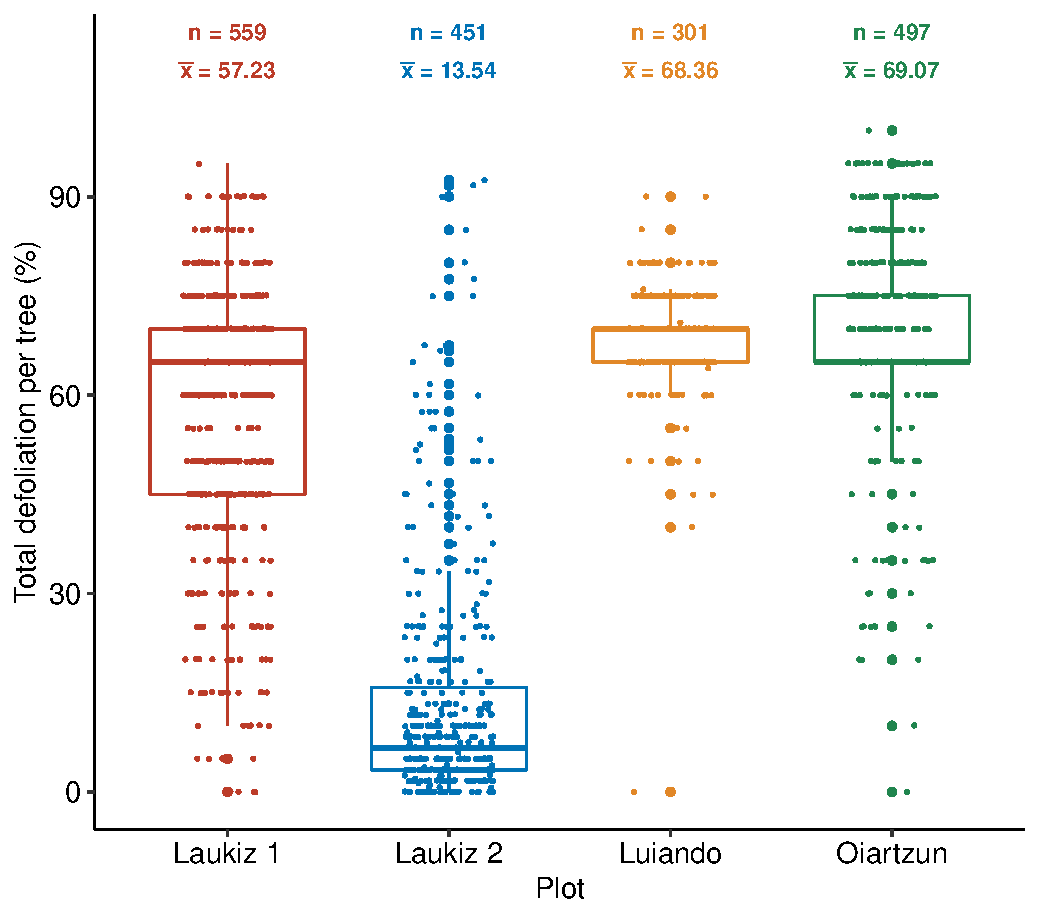
\includegraphics[width=0.48\textwidth] {defoliation-distribution-plot-1.pdf}
		\caption{Response variable defoliation at trees visualized as violin plots showing the variance of in-situ measurements for plots \textit{Laukiz 1}, \textit{Laukiz 2}, \textit{Luiando} and \textit{Oiartzun}.}\label{fig:defol-distr}
	\end{center}
\end{figure}

\subsection{In-situ data}

\noindent The \textit{Pinus radiata} plots of this study, namely \textit{Laukiz 1}, \textit{Laukiz 2}, \textit{Luiando} and \textit{Oiartzun}, are located in the northern part of the Basque Country (\autoref{fig:study_area}).
\textit{Oiartzun} has the most observations (n = 529) while \textit{Laukiz 2} features the largest area size (1.44 ha).
All plots besides \textit{Luiando} are located nearby the coast (\autoref{fig:study_area}).
In total 1759 observations are available (\textit{Laukiz 1} = 479, \textit{Laukiz 2} = 451, \textit{Luiando} = 300, \textit{Oiartzun} = 529).
The data was surveyed in September 2016.

\begin{figure} [t!]
	\begin{center}
		\centering
		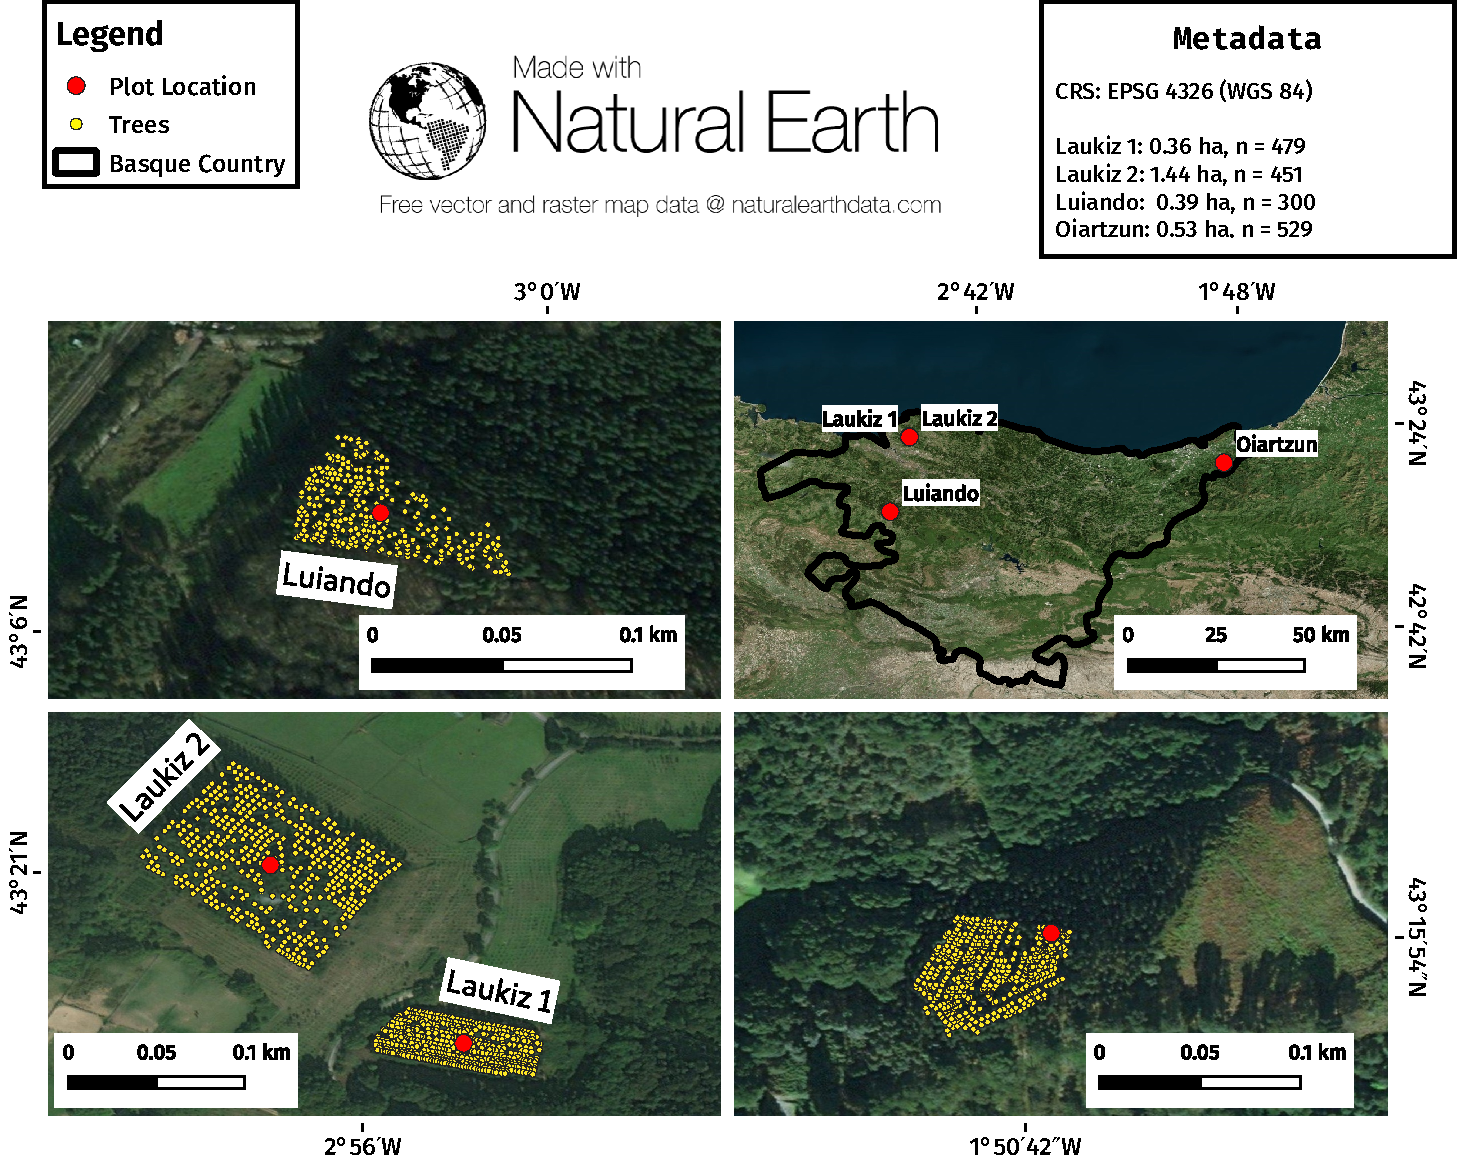
\includegraphics[width=0.48\textwidth] {study-area-hyperspectral.pdf}
		\caption{Information about location, size and spatial distribution of trees for all plots used in this study.}\label{fig:study_area}
	\end{center}
\end{figure}

%\begin{figure} [t!]
%	\begin{center}
%		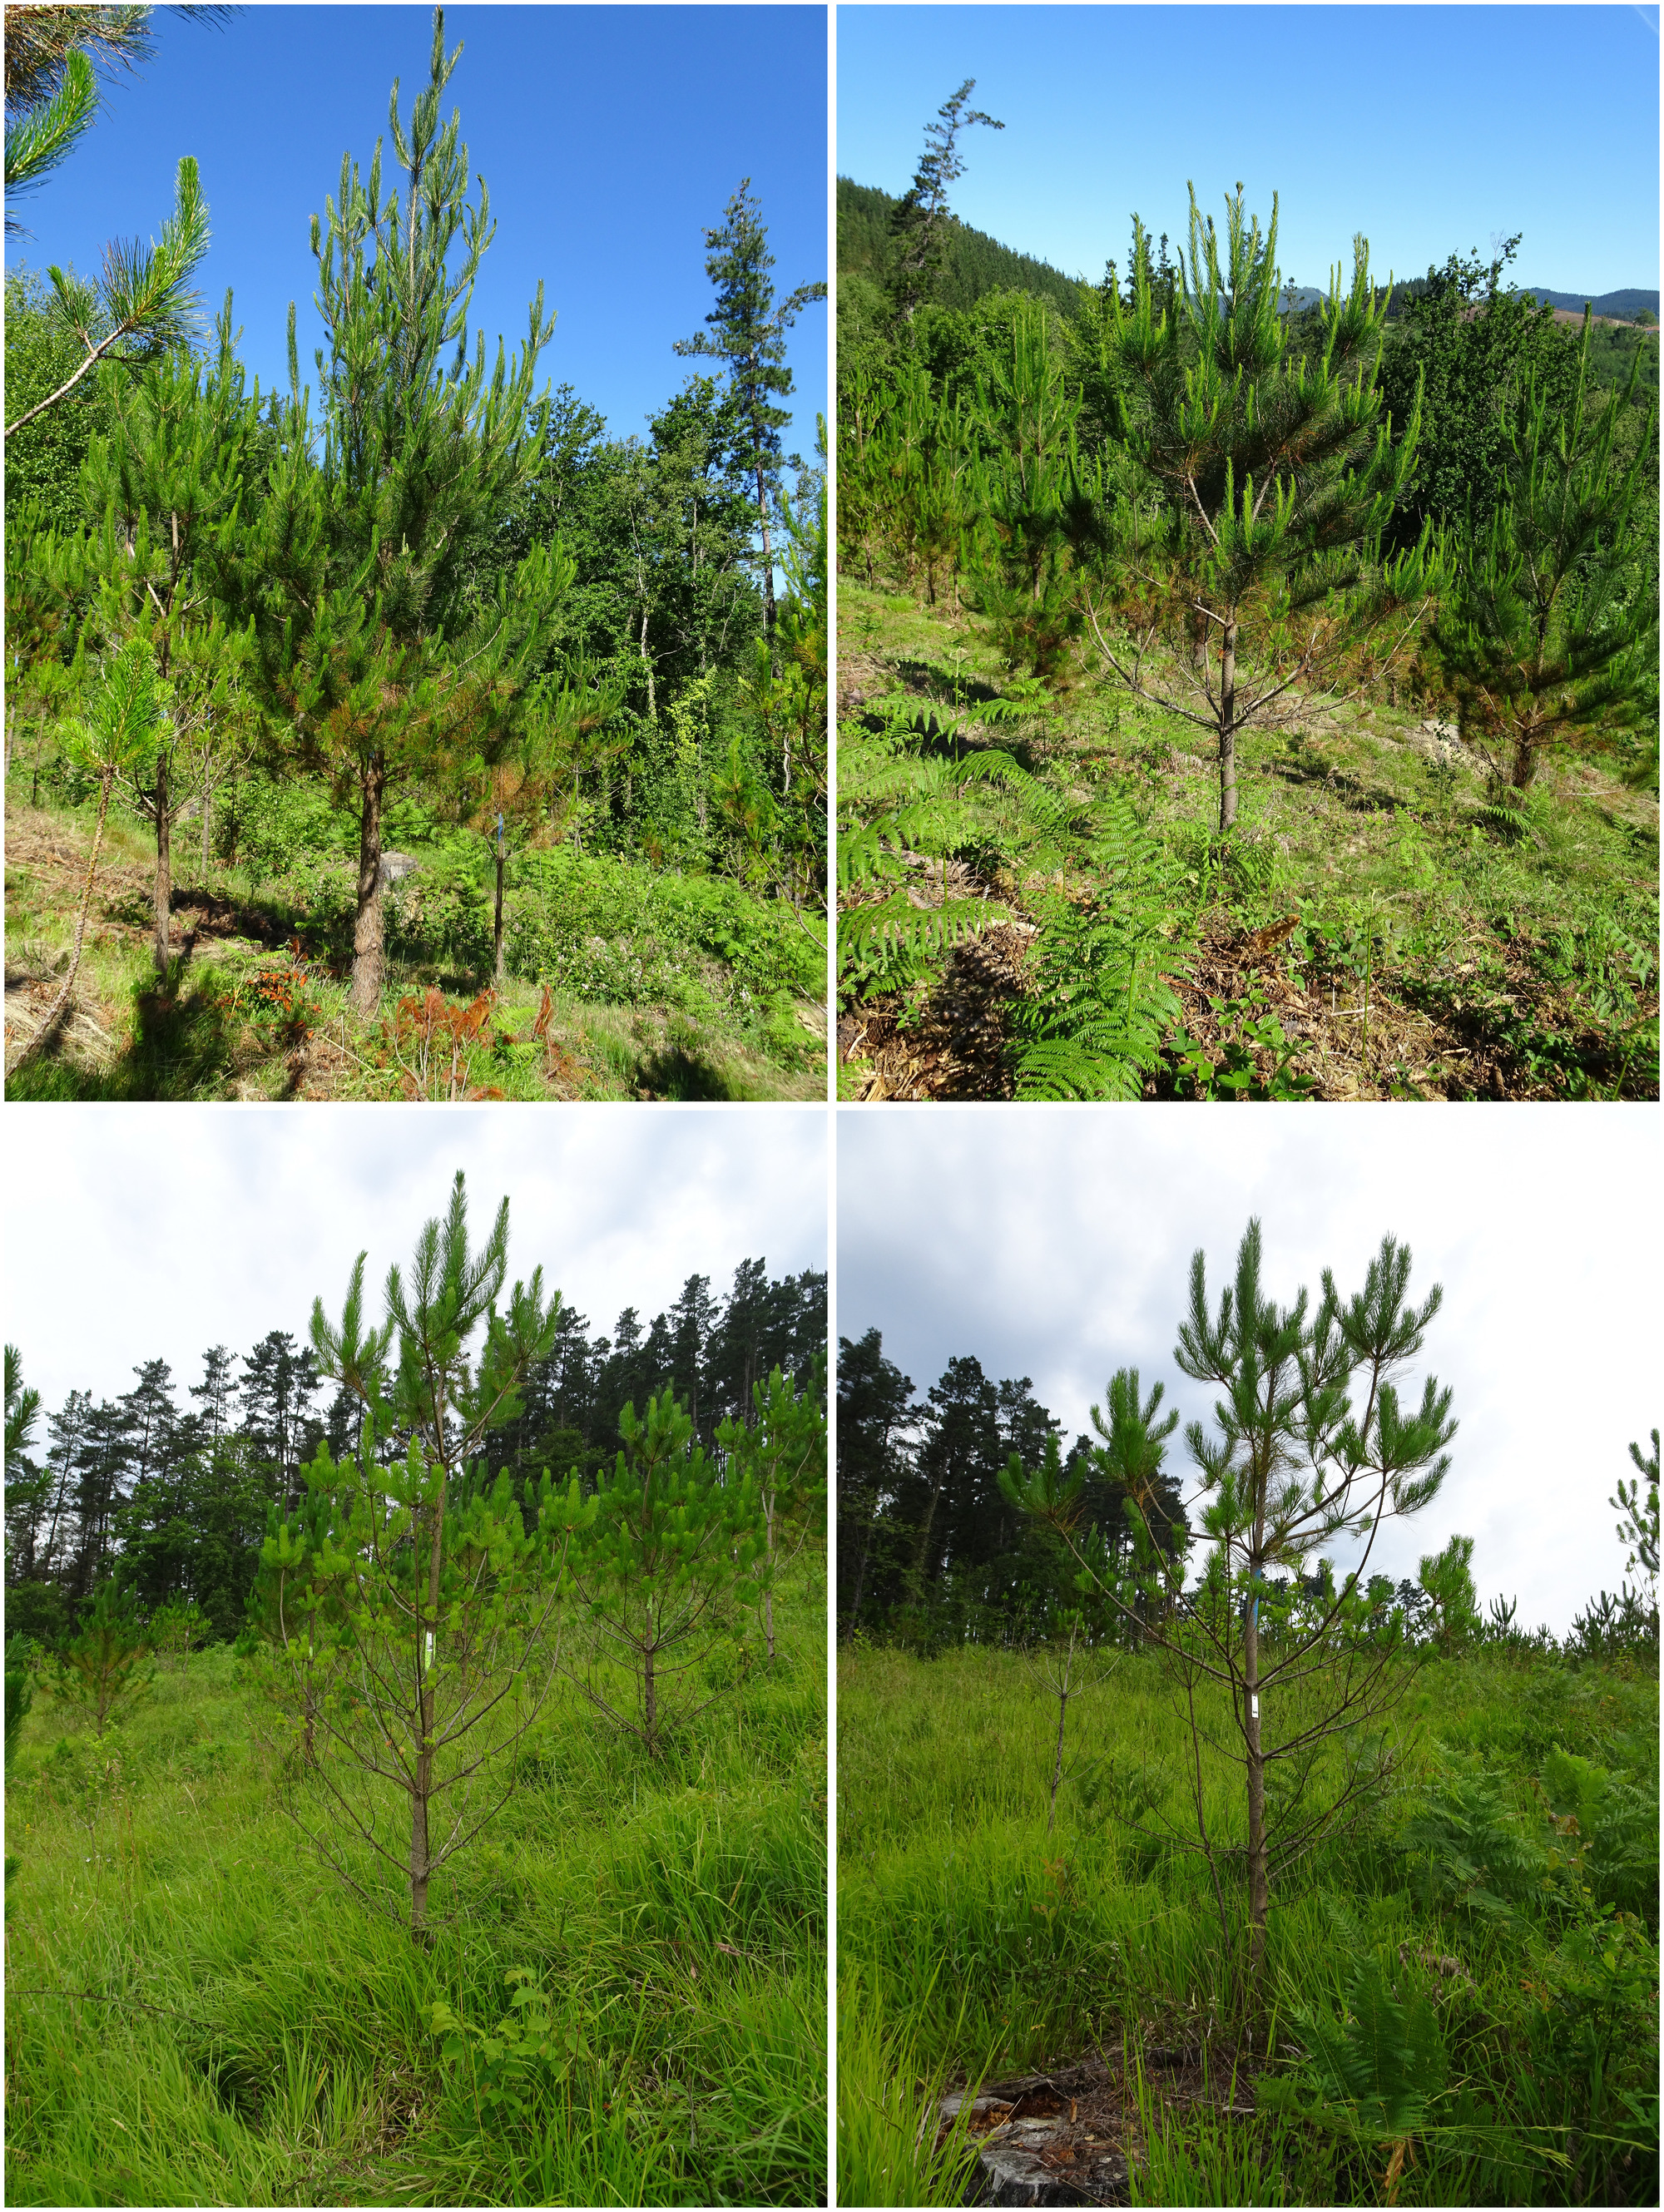
\includegraphics[width=0.48\textwidth] {defol-grid-3000px.jpg}
%		\caption{Example trees showing different levels of defoliation as interpreted by the surveyor: 10 \% (top-left), 20 \% (top-right), 40 \% (bottom-left), 60-70 \% (bottom-right).}
%		\label{fig:defol-trees}
%	\end{center}
%\end{figure}


\subsection{Hyperspectral data}

\noindent The airborne hyperspectral data was acquired during two flight campaigns on September 28th and October 5th 2016, both around 12 am.
The images were taken using a AISAEAGLE-II sensor.
All preprocessing steps (geometric, radiometric, atmospheric) have been conducted by the \ac{ICGC}.
The first four bands are corrupted, leaving 122 bands with valid information.
Additional metadata information is available in \autoref{tab:hyperparameter_limits}.

% parameter limits

\begin{table}[t]
\centering
\caption[t]{Specifications of hyperspectral data.}
\begingroup
\begin{tabular}{ll}
	\\
	Characteristic         & Value                               \\
	\toprule
	Geometric resolution   & 1 m                                 \\
	Radiometric resolution & 12 bit                              \\
	Spectral resolution    & 126 bands (404.08 nm --- 996.31 nm)   \\
	Correction:            & Radiometric, geometric, atmospheric
\end{tabular}
\endgroup\label{tab:hyperparameter_limits}
\end{table}

\section{Methods}

\subsection{Derivation of indices}
\noindent To use the full information from the hyperspectral data, all possible vegetation indices supported by the R package \textit{hsdar} (89 in total) as well as all possible \ac{NRI} combinations were calculated.
The following formula was used for the NRI calculation:

\begin{equation}
	NRI_{i,j} = \frac{b_{i} - b_{j}}{b_{i} + b_{j}}
\end{equation}

\noindent
where \(i\) and \(j\) are the respective band numbers.

\bigbreak{}

\noindent To account for geometric offsets (which were reported with up to 1 m from \ac{ICGC}), a buffer of two meters around the centroid of the respective tree was drawn.
The value assigned to a tree observations was the mean of all pixels which touched the respective buffer around the tree.
In total, \(\frac{125*126}{2} = 7875\) NRIs were calculated.
Due to four corrupted bands of the sensor a total of 7471 indices were available for each observation.

\subsection{Dimension reduction}

\noindent It is important to distinguish the term 'dimension reduction' from 'high-dimensionality'.
The former refers to the general idea of reducing features from a dataset\cite{vandermaaten2007}.
In modeling this means finding the best subset of covariates which provide the most predictive power to the model or extracting the main components of the features using a \ac{PCA}.
'High-dimensionality' in contrast is defined as a dataset attribute and applies
when \(p > n\), where \(p\) is the number of covariates and \(n\) the number of
observations\cite{hastie2001}.
There is no absolute value at which the term can be applied, both for \(n\) and \(p\).
Hence for this study the word ‘high-dimensionality‘ only applies to the
experiments using the ‘NRI‘ feature set (7470 features for 1759 observations).

The case of a feature-rich dataset comes with several challenges for both model fitting and evaluation.

\begin{itemize}
	\item Model fitting times increase
	\item Noise is possibly introduced into models by highly-correlated variables\cite{johnstoneiainm.2009}
	\item Model interpretation and prediction tasks become more complicated\cite{johnstoneiainm.2009}
\end{itemize}

\noindent In the following sections a brief overview about sub-categories of feature-selection approaches is given.
Due to the focus of this study on the use of filter methods, all other approaches were grouped into a single section.

\subsubsection{Filter methods}

% Filter methods
\noindent The concept of 'Filter methods' originates on the idea of ranking features using certain heuristics of an algorithm\cite{chandrashekar2014}.
Some filter methods are restricted towards specific types of variables (numeric or nominal data).
After the covariates have been ranked, a decision needs to be made what features to keep and which to discard\cite{drotar2015}.
This step is usually done within the optimization phase of the model fitting, along with the hyperparameter tuning.
Essentially, the number of covariates in the model is treated as a hyperparameter of the model.
The goal is to optimize the number of features (using the ranked covariates) at which the model achieves the best performance.
In well-implemented software solutions the filter calculation is only done once
and then cached, saving valuable resources\cite{mlr}.

\paragraph{Ensemble filter methods}

% Ensemble filter methods
Besides the concept of choosing a specific filter method to rank variables,
studies showed that combining several filters using statistical operations such
as 'minimum', 'mean' or 'sum' are able to enhance the predictive performance of
the resulting models\cite{abeel2010, drotar2017a}.
This approach is referred to as 'ensemble filter'\cite{dietterich2000}.
Ensemble filters align with the recent rise of the 'ensemble' approach in machine-learning which uses stacking to combine the predictions of multiple models, aiming to enhance predictive performance\cite{polikar2012, feurer2015}.
In this work the 'Borda' ensemble filter was applied\cite{drotar2017a}.
The final order is the sum of all single filters ranking.

\paragraph{Ensuring a fair weighting in the ensemble}

Filter methods can be grouped into classes: Correlation based, entropy based, linear and non-linear methods.
It is important to not give certain classes too much weight in the ensemble as otherwise the final result will be biased.
This was taken care of by calculating the rank correlations (Spearman's correlation) of the generated feature rankings of all methods against each other.
In case filters showed high correlations with each other, these were not included into the ensemble filter.
This ensures that the ensemble filter is not biased towards a certain group of methods yielding highly similar rankings.

\paragraph{Description of used filter methods}

Filter methods can be classified as follows:

\begin{itemize}
	\item univariate/multivariate (scoring based on a single variable / multiple variables)
	\item linear/non-linear (calculation of linear/non-linear interaction terms)
	\item entropy/correlation (scoring based on derivations of entropy or correlation based approaches)
\end{itemize}

% filter methods
\begin{table}[b!]
\centering
\caption[t]{List of filter methods used in this work}
\begingroup\footnotesize
\begin{adjustbox}{width={0.48\textwidth},totalheight={\textheight},keepaspectratio}
	\begin{tabular}{lll}
		\\
		Name                                         & Group                             & Reference          \\
		\toprule
		Linear correlation (Pearson)                 & univariate, linear, correlation   &\cite{pearson1901} \\
		Information gain                             & univariate, non-linear, entropy   &\cite{quinlan1986} \\
		Minimum redundancy, maximum relevance        & multivariate, non-linear, entropy &\cite{zhao2013}    \\
		Carscore                                     & multivariate, linear, correlation &\cite{zuber2011}   \\
		Relief                                       & multivariate, linear, entropy,    &\cite{kira1992}    \\
		Conditional minimal information maximization & multivariate, linear, entropy     &\cite{fleuret2004}
	\end{tabular}
\end{adjustbox}
\endgroup\label{tab:filter-methods}
\end{table}

\noindent Filter method 'information gain' is only defined for nominal response variables:

\begin{equation}
	H(Class) + H(Attribute) - H(Class, Attribute)
\end{equation}

where \(H\) is the conditional entropy of the response variable (class) or the feature (attribute), respectively.
To be able to use this method with a numeric response, the variable is discretized into equal bins and treated as a class variable.
While the number of bins can be treated as a hyperparameter of the filter method, we decided to use \texttt{\(n_{bin}\) = 10} after rank correlations of > 0.9 for different bin sizes were observed in a side analysis.

\subsubsection{Wrapper methods and PCA}

\noindent Other approaches to assess feature importance are 'wrapper methods' and the \ac{PCA}\cite{das2001, jolliffe2016}.
A short introduction to both is given below.

% Wrapper approach
\noindent 'Wrapper methods'\cite{chandrashekar2014, kohavi1997} apply algorithms that are used for hyperparameter optimization such as 'Random Search' or 'Generic Simulated Annealing'.
First a (random) subset of features is chosen based on the selected algorithm.
In comparison to 'filters', no ranking is done in this step.
Now the model is fitted on the data and the performance is evaluated.
This is done multiple times, depending on the defined stopping criteria set by the user (performance, runtime, evaluations).
A disadvantage of this approach is that hyperparameter tuning can only be applied after the feature-selection optimization finished.
Hence, the 'wrapper approach' is an expensive optimization method because two stages need to be run in sequential order.
Due to their extensive runtimes, 'wrapper methods' were not considered in this work.

% PCA
A method with a completely different approach compared to filters and wrappers is the 'Principal Component Analysis'\cite{pearson1901, jolliffe2016}.
Here, the main components of the feature space are extracted and combined.
Most often the first two extracted main components are used since these contain the major information of the covariates.
By using the (automatically estimated) explained variance of the main components, the model can rely on a few features containing the majority of information available in the data.
This enables cheap model fitting with balanced loss of predictor information.
The disadvantage of this methodology is the lack of interpretability because the main components cannot be related back to the original covariates.


\subsection{Benchmarking design}


\subsubsection{Algorithms}

\noindent The benchmarking matrix of this study consists of the following algorithms:

\begin{itemize}
	\item  Extreme Gradient Boosting (XGBOOST)
	\item  Random Forest (RF)
	\item  Penalized Regression (both L1 and L2)
	\item  Support Vector Machine (SVM)
\end{itemize}


\noindent \ac{RF} and {SVM} are well established algorithms that are widely used in environmental modeling.
Extreme gradient boosting (commonly referred to as \ac{XGBOOST}) showed promising results in benchmark competitions in recent years.
Penalized regression is a statistical modeling technique capable of dealing with highly-correlated covariates by applying a penalization term which shrinks the coefficients of the model\cite{hastie2001}.
Common penalties are 'lasso' (L1) and 'ridge' (L2).
The former does not allow the full removal of variables from the model (penalization to zero) while the latter does.
Both penalties can also be combined.
The combined approach is called 'elastic net' but was not used in this work.

\subsubsection{Feature sets}
% TODO: talk about the reasons behind different features sets: environmental implications

\noindent Three feature sets were used in this study with each representing a different way of feature-engineering:


\begin{itemize}
	\item The raw hyperspectral band information (HR: No feature engineering) %chktex 13
	\item Vegetation Indices (\ac{VI}: Expert-based feature engineering)
	\item Normalized Ratio Indices (\ac{NRI}: Automated feature-engineering)
\end{itemize}

\subsubsection{Hyperparameter Optimization}

\noindent An exhaustive hyperparameter tuning was applied during nested spatial \ac{CV} for all algorithms.
Maximum Bayesian Optimization\cite{mlrmbo} (MBO) was used for parameter optimization.
This approach first composes \textit{n} randomly chosen hyperparameter settings out of a user defined search space.
After these \textit{n} tries have been evaluated, a new hyperparameter setting, which is going to be evaluated next, is proposed based on a fitted regression model.
The regression model estimates the performance of the machine-learning method for unknown hyperparameter settings.
Using these estimates, a new promising hyperparameter setting is proposed to be evaluated next.
This strategy continues until a termination criterion, defined by the user, is reached\cite{hutter2011, jones1998}.
An initial design of 30 randomly composed hyperparameter settings and a termination criterion of 70 iterations was used, resulting in a total budget of 100 evaluated hyperparameter settings per fold.
The advantage of this tuning approach is the substantial reduction of the tuning budget required to find a setting which is close to the global minimum
This applies when being compared to methods that do not use information from previous runs, such as random search or grid search\cite{bergstra2012}.
In addition to MBO, the penalization term of Lasso and Ridge was optimized using the internal non-spatial CV approach due to promising results in other applications.

For the filter methods, the percentage of features was added to the models as a hyperparameter.
The number of main components was tuned for the instances which used \ac{PCA} instead of filtering.
Random Forest hyperparameter \texttt{\(m_{try}\)} was transformed from taking absolute values to a relative parameter depending on the number of tasks: \(p^{m_{try}}\), where \(p\) is the number of features.
This was necessary to ensure that \texttt{\(m_{try}\)} was not chosen out of bounds during tuning:
After the filtering, only a subset of features of the task is used for optimizing the models hyperparameters.
The size of this subset is always different since the number of features is also optimized.
Hence, the value of  \texttt{\(m_{try}\)} needs to be created flexible based on the number features.

\subsubsection{Spatial resampling}

\noindent A spatial block nested cross-validation was chosen to reduce the influence of spatial autocorrelation as much as possible\cite{schratz2019, sperrorest}.
Each plot served as one fold within the resampling setup, resulting in four folds total.
For the inner level (hyperparameter tuning), \(p - 1\) folds were used (with \(p\) being the number of plots).

In total the benchmarking matrix consisted of 120 experiments (3 feature sets, 5 algorithms, 8 feature-selection methods).

\subsection{Calculation of model feature importance}
\noindent A permutation-based feature importance estimation was conducted for the best algorithm of each feature set and filter method, respectively.
This method calculates the loss of predictive performance for each feature by permuting it in a random manner.
The more important the feature is for the model, the higher the loss in the used error measure will be, reflecting the importance of the specific feature for the current model.
To balance both runtime and variance reduction, we opted for 25 iterations of each feature permutation.

\subsection{Linking feature importance to wavelength regions}
\noindent For ecological interpretation purposes we linked the ten most important indices of the winning models for each feature set to the spectral regions of the hyperspectral data.
For feature set HR and NRI a direct linking to the respective bands of the hyperspectral sensor was done.
For the vegetation indices all bands covered by the spectral range of calculated vegetation indices were counted and summed up.

\subsection{Research compendium}

\noindent The complete study was done using the open-source statistical programming language R\cite{rcoreteam2018}.
The algorithm implementations of the following packages have been used: \textit{xgboost}\cite{chen2016} (\textit{xgboost}), \textit{kernlab}\cite{kernlab} (Support Vector Machine) and \textit{glmnet}\cite{glmnet} (Ridge Regression).
The filter methods of the following packages were used: \textit{praznik\cite{praznik}}, \textit{FSelectorRcpp}\cite{fselectorrcpp}.
The R package \textit{mlr}\cite{mlr} was used for all modeling related steps.
\textit{drake} was used for structuring the work and ensuring reproducibility.
This study is available as a research compendium on Zenodo (\url{10.5281/zenodo.2635403}).


\section{Results}

\subsection{Predictive performance}

% - RMSE around 34
% - MBO tuned penalized methods are substantially worse
% - Carscore, Info und Borda were at least once among the best combination for a learner
\noindent No practical differences in RMSE were observed among the feature sets (\autoref{fig:perf-result}).
SVM showed the lowest error in four out of six tasks.
Overall, the response variable 'defoliation at trees' could be modeled with an error of 34 \%.

% tasks
% - no substantial difference between feature sets
% - combining feature sets makes no difference
% - expert based feature sets show no better result than data-driven ones
% - penalized methods seem to have problems with VI feature set
No practical difference was observed between feature sets.
The combination of feature sets showed no increase in performance.
All learners scored evenly across all tasks.
Feature sets containing expert-based variables (VI) showed no substantial difference to data-driven tasks (NRI).

% learner
% - RF Car is the overall winner
% - Ridge-CV hit and miss (hit = NRI, miss = VI)
% - all MBO penalized methods have no difference across tasks
Random Forest combined with the 'Carscore' filter showed the best absolute performance (RMSE of 3.396) (\autoref{tab:perf-top-15}).
A noticeable difference between SVM and all other learners was visible for all
feature sets without NRI variables (difference in RMSE of 3 --- 4).
Considering a grouped performance by learners across all tasks and filters, SVM showed the most robust results (\autoref{tab:perf-top-15}).
L1 penalized regression showed slightly better results in three out of six tasks when being optimized using the package internal 10-fold CV compared to MBO (RMSE of 50 vs 58).
Regression with Ridge penalty (L2) showed a high variance when comparing results across tasks: In three out of six tasks (all including VI variables) the error was out of bounds (HR-NRI-VI\@; HR-VI, VI), for HR-NRI and HR the error was medium (around 40 RMSE), and for task NRI Ridge regression achieved almost the same score as the best performing model (3.39 RMSE, NRI) (\autoref{tab:perf-top-15}).
All penalized methods tuned using MBO showed exactly the same error across all tasks.

% filters
% - influence varies based on algorithm and task (SVM very small influence, RF medium, XGB medium)
% - no substantial decrease in performance when using filters
% - no advantage of ensemble borda filter compared to others
Effects of filter methods on performance differed between algorithms:
With the exception of one or two methods, SVM showed a constant performance of all filters across tasks (\autoref{fig:filter-perf-all}).
RF showed a normal distribution for most tasks with one or two different methods taking the lead on each task.
For RF, filter 'Carscore' showed the best performance in three out of six tasks while this was achieved for XGBoost by filter 'CMIM'.
XGBoost showed a diverse distribution with less clustering of filters as SVM and RF (referring to RMSE).

% filter vs no filter
When comparing the usage of filters vs using no filter at all, there was only one instance (XGBoost on the HR-NRI task) when the model with no filtering showed a slighly better performance than the best filtered one (\autoref{fig:filter-effects}).
In general, the effect of filtering vs.\ no filtering differed without a clear pattern across tasks: For example, SVM and RF showed a substantial increase for the NRI task when filtering the data while there was almost no effect for XGBoost (\autoref{fig:filter-effects}).
For task HR, there was a medium effect of applying filtering for RF, almost none for SVM and a large one for XGBoost.

% latex table top 20 absolute performances
% latex table generated in R 3.6.1 by xtable 1.8-3 package
\begin{table}[ht!]
\centering
\caption{Top 15 results for any task/learner/filter combination, sorted by performance.} 
\label{tab:perf-top-15}
\begin{tabular}{rlllrr}
  \hline
 & Task & Model & Filter & RMSE & SE \\ 
  \hline
1 & HR & XGBoost & CMIM & 30.83 & 13.90 \\ 
  2 & HR-NRI & XGBoost & Info & 31.03 & 15.96 \\ 
  3 & HR-NRI-VI & XGBoost & CMIM & 31.17 & 14.78 \\ 
  4 & HR & RF & MRMR & 31.44 & 15.08 \\ 
  5 & HR & XGBoost & Relief & 31.44 & 15.08 \\ 
  6 & HR & XGBoost & MRMR & 31.44 & 15.08 \\ 
  7 & HR-NRI-VI & SVM & Relief & 31.58 & 15.60 \\ 
  8 & NRI & SVM & Car & 31.61 & 15.58 \\ 
  9 & HR-NRI-VI & RF & Car & 31.64 & 14.89 \\ 
  10 & HR-NRI-VI & SVM & Info & 31.67 & 15.49 \\ 
  11 & NRI & SVM & Borda & 31.70 & 15.46 \\ 
  12 & VI & SVM & Pearson & 31.75 & 15.08 \\ 
  13 & HR-NRI & SVM & Relief & 31.78 & 15.39 \\ 
  14 & NRI & SVM & Info & 31.80 & 15.37 \\ 
  15 & VI & SVM & CMIM & 31.81 & 15.51 \\ 
   \hline
\end{tabular}
\end{table}


% latex table best performance per learner
% latex table generated in R 3.6.1 by xtable 1.8-3 package
\begin{table}[ht!]
\centering
\caption{Best performance of each learner across any task and filter method.} 
\label{tab:best-learner-perf}
\scalebox{0.9}{
\begin{tabular}{rlllrr}
  \hline
 & Task & Model & Filter & RMSE & SE \\ 
  \hline
1 & NRI & SVM & Info Gain & 27.99 & 19.15 \\ 
  2 & NRI & RF & Car & 30.77 & 16.86 \\ 
  3 & VI & Lasso-MBO & No Filter & 31.01 & 14.71 \\ 
  4 & HR-NRI-VI & XGBoost & Borda & 31.05 & 17.01 \\ 
  5 & NRI & Ridge-MBO & No Filter & 31.16 & 15.03 \\ 
   \hline
\end{tabular}
}
\end{table}


% plot performance results
\begin{figure} [t!]
	\centering
	\begin{center}
		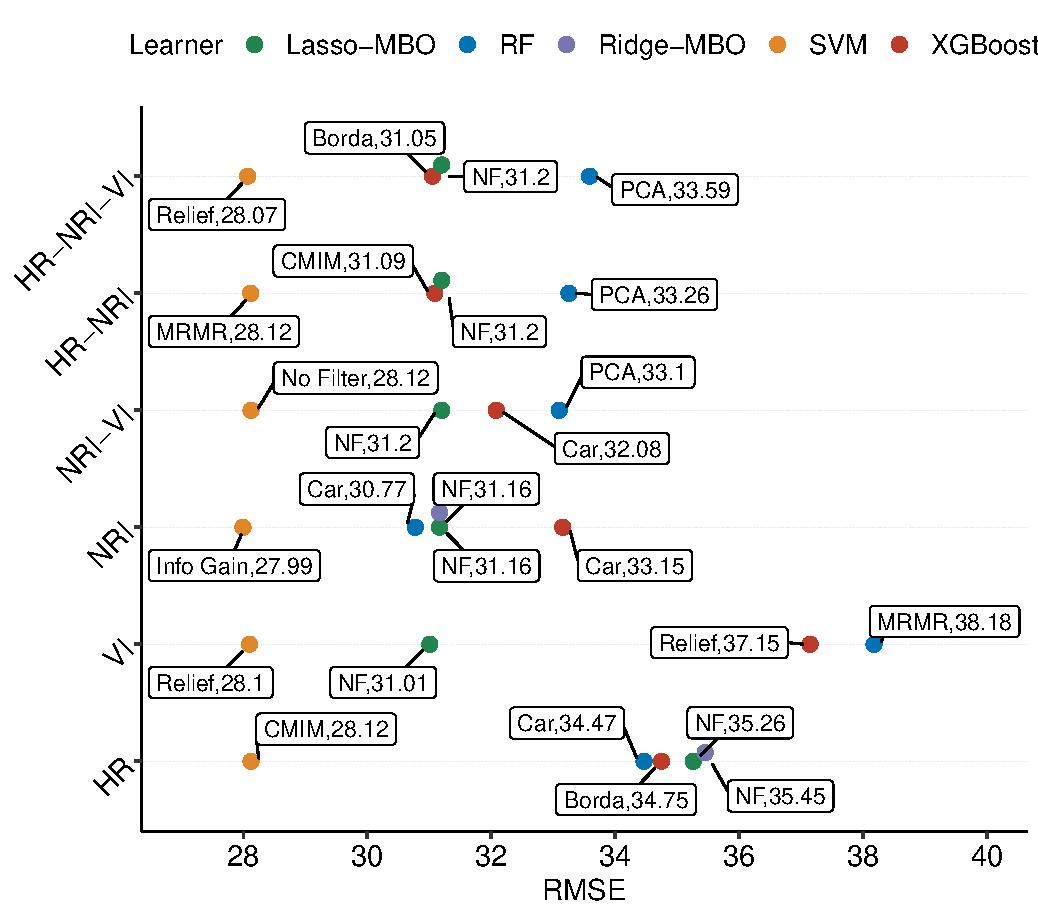
\includegraphics[width=0.48\textwidth] {performance-results-1.pdf}
		\caption{Scored predictive performance (RMSE) of models across tasks. Prefix 'CV' denotes that the learner was optimized using internal 10-fold CV while prefix 'MBO' means that Bayesian optimization was used for hyperparameter optimization. The abbreviations on the y-axis refer to the combinations of feature sets on which each model was scored on. Labels attached to each point in space show which filter method was used for scoring features during the feature selection process (NF = no filter, Car = 'Carscore', Info = 'Information Gain', Borda = 'Borda'). The second value in the attached label of each point shows the scored RMSE value of the respective setting.}\label{fig:perf-result}
	\end{center}
\end{figure}

% plot no filter vs best filter for each model and task
\begin{figure} [t!]
	\centering
	\begin{center}
		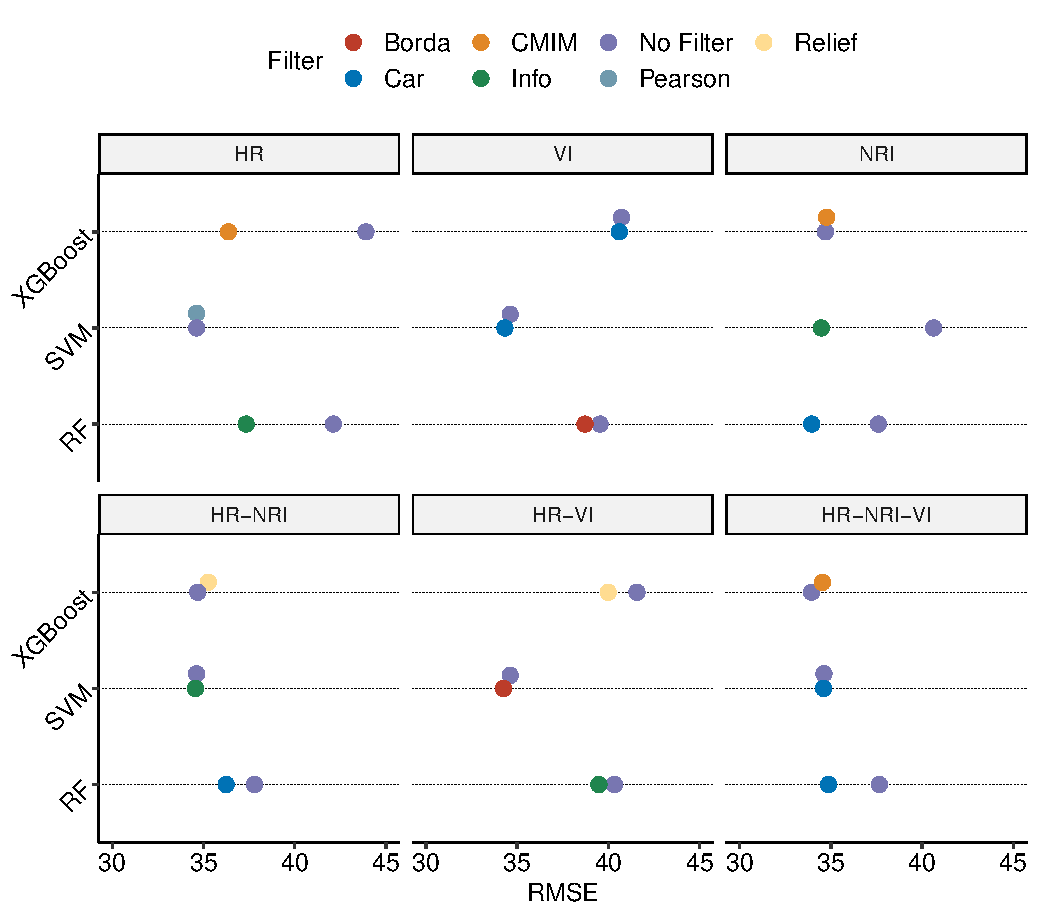
\includegraphics[width=0.48\textwidth] {filter-effect-1.pdf}
		\caption{Model performances in RMSE when using no filter method compared to the best scoring filter method for each learner across all tasks.}\label{fig:filter-effects}
	\end{center}
\end{figure}
\subsection{Permutation-based variable importance}

% plot no filter vs best filter for each model and task
\begin{figure} [t!]
	\centering
	\begin{center}
		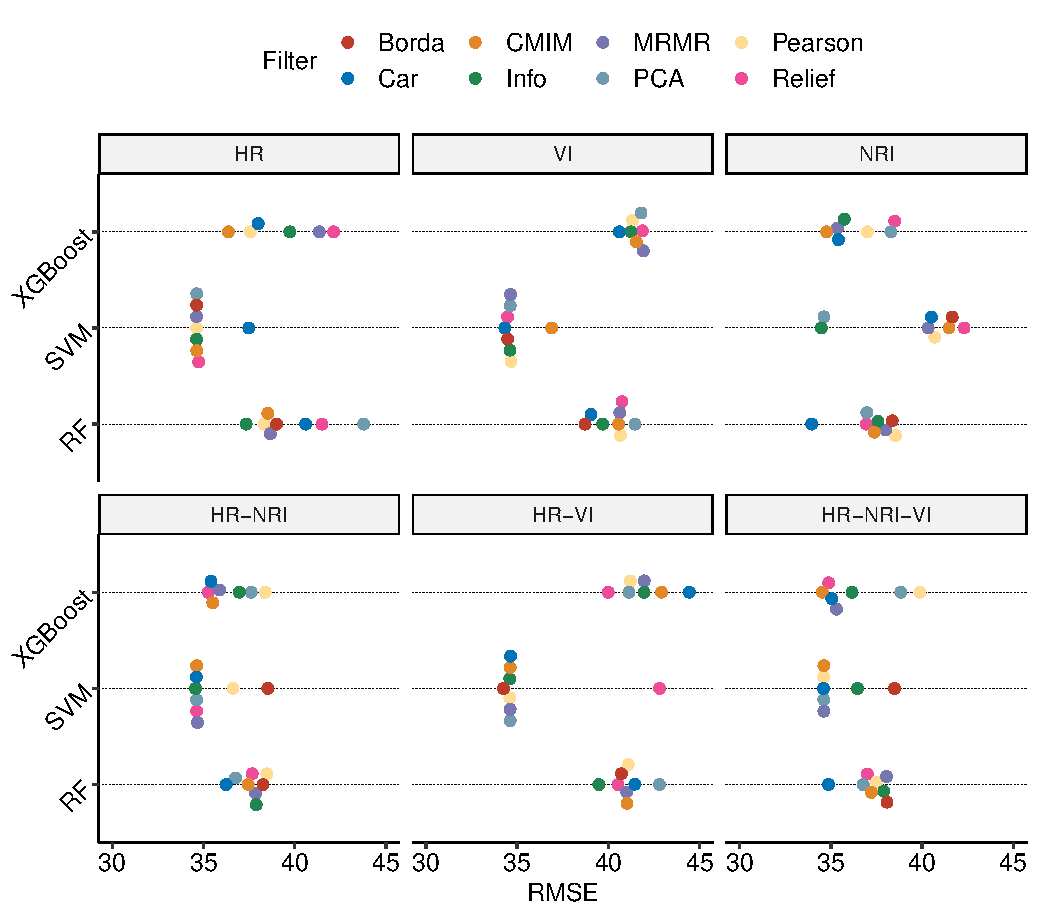
\includegraphics[width=0.48\textwidth] {filter-perf-all-1.pdf}
		\caption{Model performances in RMSE of all used filter methods and PCA for each learner across all tasks.}\label{fig:filter-perf-all}
	\end{center}
\end{figure}


\subsection{Permutation-based variable importance}
\section{Discussion}

\subsection{Derivation of indices}

\noindent The decision to use a buffer of 2 m to generate the index value for each observation is questionable.
When using no buffer at all, the possibility is high that a pixel value gets assigned to a tree which does not spatially match with the actual recorded hyperspectral reflectance due to the geometric offset of 1 m.

Using a buffer of more than 2 meters increases the probability of including information from other trees into the pixel value, blurring the actual value of the tree observation.
In our view using a buffer of 2 m is a good compromise between both worlds.

Another critical point is that the exact number of contributing pixels to the final index value of an observation cannot be determined as it depends on the location of the tree within the pixel grid.
As the buffer is circular, determining the total number of contributing pixels depends on the exact location of a tree within that pixel as this sets the base how many pixels in each direction will be touched by the buffer.
If a tree observation is located at the border of the plot, some directions of the buffer will contain no values and the subsequent index value will be calculated using less pixels than if the tree observation is located in the middle of the plot.

The magnitude of bias introduced by these facts cannot be quantified.
However, it has to be considered when making interpretations about the outcome of this study.

\subsection{Performance vs.\ plot characteristics}
% TODO: Really needed?

\subsection{Predictive Performance}

\subsubsection{Algorithm differences}

\subsubsection{Feature set differences}

\subsection{Feature selection methods}

% - Ensemble FS show no advantage to simple methods -> maybe to less features, features too correlated? check diff between effect on NRI and VI
% - Effect varies across learners -> suggest to use FS even on feature sets with p < 100?
% - When calculating multiple filters, consider to only use ensemble filter?
% - PCA shows similar performance but probably requires tuning of main components -> check runtime!

\subsubsection{Variable importance vs.\ filter methods}

WIP

\subsubsection{Ecological Interpretation}

% TODO: talk about the link to RS spectra

\subsection{Comparison to other studies}
% NOTE: no environmental studies use filter methods, some use FFS
% NOTE: only few studies analyze defoliation

\noindent Most other studies analyzing defoliation operated on the plot rather than the tree level.
This originated simply due to spatial resolution of the satellite products that served as the input data\cite{townsend2012, debeurs2008, rengarajan2016}.

Studies focusing on tree-level defoliation used ground-level methods such as \ac{ALS} or \ac{LiDAR}\cite{meng2018, kalin2019}.
\~cite{meng2018} used \ac{OLS} regression methods while\cite{kalin2019} retrieved information out of ground-level RGB photos using \ac{CNN}.
Both study designs are substantially different compared to the setup of this work.
In addition, no spatial \ac{CV} or \ac{FS} was used.
\~cite{goodbody2018} used a \ac{PLS} model with high-resolution \ac{DAP} to predict cumulative defoliation caused by the spruce budworm.
Study results indicated that spectral metrics were found to be most helpful for the model.
Incorporating such metrics (both spectral and structural) could be a possible enhancement for future works.

\~cite{shendryk2016, ludwig2019} are studies which are more similar in their methodology but focus on a different response variable.
\~cite{shendryk2016} used machine-learning models with \ac{ALS} data to study dieback of trees for eucalyptus forests.
A grid-search was used for hyperparameter tuning and a \ac{FFS} for variable selection.
\~cite{ludwig2019} analyzed woody cover in South Africa using spatial \ac{CV} and a relatively novel spatial \ac{FS} approach\cite{meyer2018} on a Random Forest classifier.

In summary, we could not find studies using filter methods for \ac{FS} or \ac{NRI} indices in their work with a relation to forest health.
Most studies used only one algorithm (usually Random Forest) without strong arguments why this particular one has been selected.
In our view the number of possible derivable input features is often higher than the actual number of variables used in the end, missing out on potentially helpful information from the raw data.
These findings underline the importance of this work in the field of forest health modeling.

\section{Outlook and conclusion}

\appendices{}

\section{Spectral signatures of each plot}

\begin{figure} [ht]
	\begin{center}
		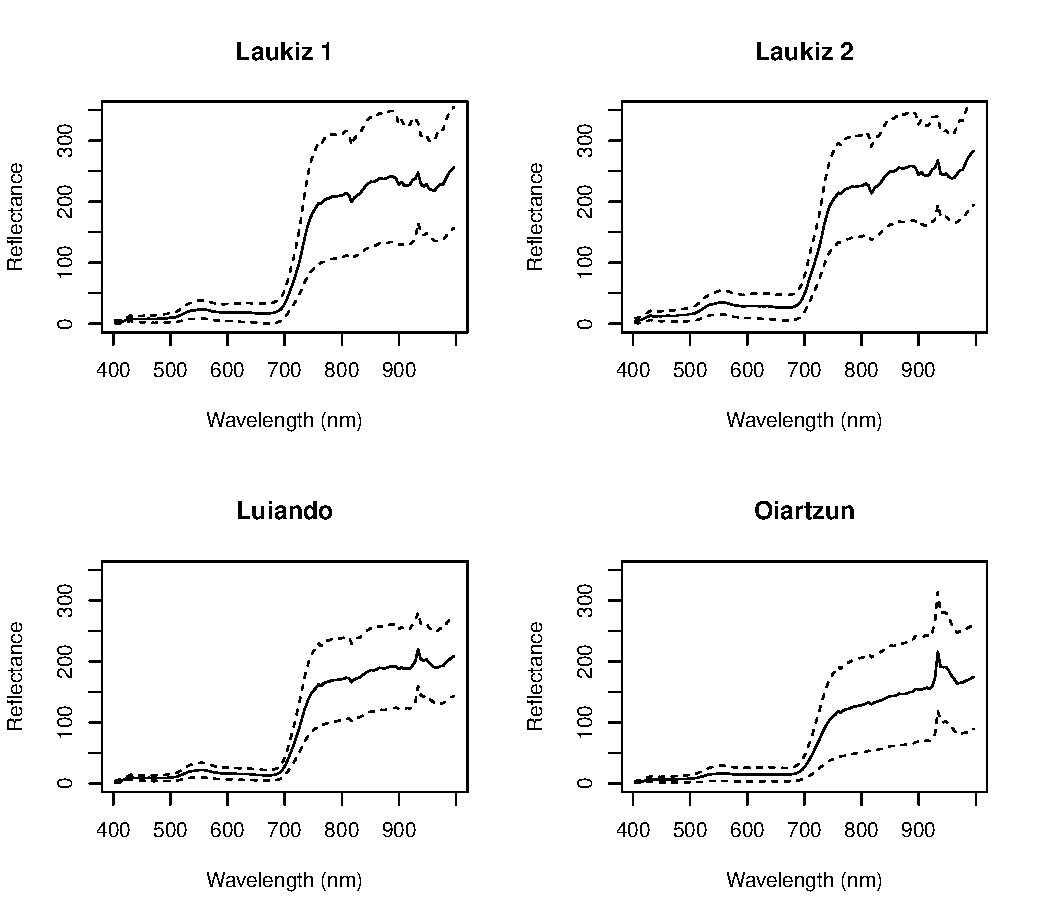
\includegraphics[width=0.48\textwidth] {spectral-signatures-1.pdf}
		\caption{Spectral signatures (mean and standard deviation) of Laukiz1, Laukiz2, Luiando and Oiartzun.}\label{fig:spectral-signatures}
	\end{center}
\end{figure}

\pagebreak

\section{Correlation among filter methods}

\begin{figure} [ht]
	\begin{center}
		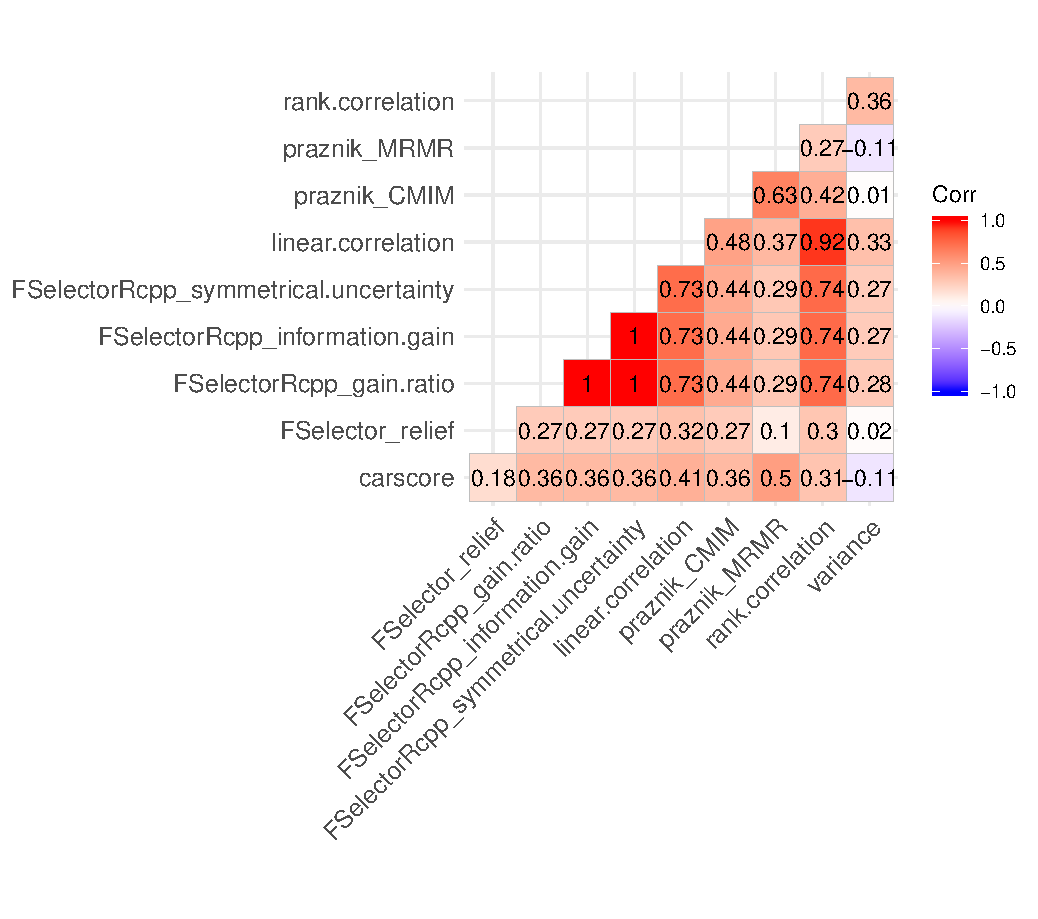
\includegraphics[width=0.48\textwidth] {correlation-filter-nri-1.pdf}
		\caption{Spearman correlation of filter rankings between various filter methods. Results of the NRI feature set are shown.}\label{fig:correlation-filters}
	\end{center}
\end{figure}

\section{Effect of different \texorpdfstring{\(n_{bins}\)}{nbins} values on filter 'information gain'}

\begin{figure} [ht]
	\begin{center}
		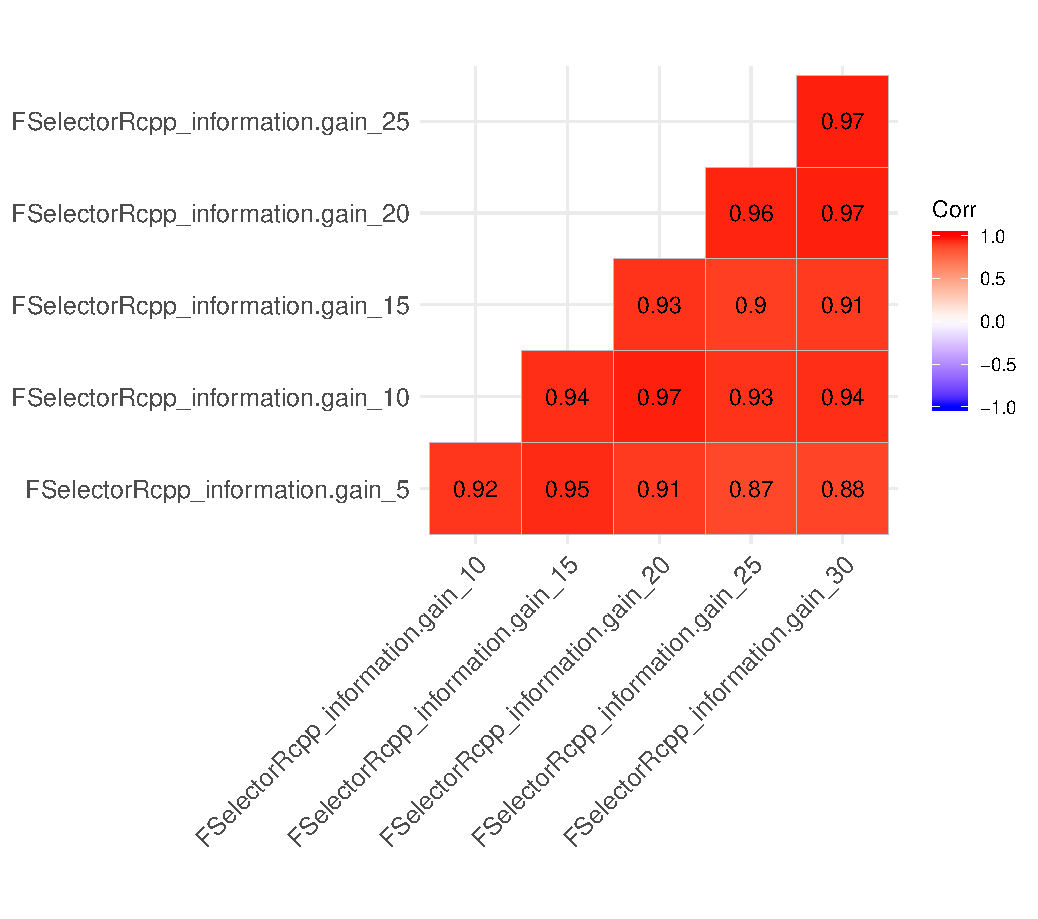
\includegraphics[width=0.48\textwidth] {correlation-nbins-1.pdf}
		\caption{Spearman correlation of filter information gain using different \texttt{\(n_{bins}\)} values for discretization of the numeric response.}\label{fig:correlation-nbins}
	\end{center}
\end{figure}



\bibliographystyle{IEEEtran}
\bibliography{Biblio}

\section*{References}

\end{document}

